\section{Ingestion module for the OPHKTM file}

This sections describes the ingestion module for inserting the production information of the package, which contains the housekeeping telemetry received from the satellite, generated by \acrshort{pdgs} to be sent to \acrshort{fos}.

The associated ingestion processors are:

\begin{itemize} 

\item \textbf{s2boa.ingestions.ingestion\_ophktm.ingestion\_ophktm}
  
\end{itemize}

This module uses the following \acrshort{dim} signatures:

\begin{itemize} 

\item \textbf{HKTM\_PRODUCTION\_VGS}: production information of the package, which contains the housekeeping telemetry received from the satellite, generated by \acrshort{pdgs} to be sent to \acrshort{fos}.
  
\end{itemize}

The table \ref{tb:description_explicit_reference_ingestion_ophktm} shows the description of the explicit references inserted by the ingestion.

\begin{longtable}{|M{0.3\linewidth}|M{0.55\linewidth}|}
\hline \textbf{Reference} & \textbf{Description} \\ \hline
\textbf{HKTM PRODUCT\_ID} & Identifier of the package generated by \acrshort{pdgs} containing the telemetry to be sent to \acrshort{fos} \\ \hline
\caption{Table describing the explicit reference associated to the ingestion}
\label{tb:description_explicit_reference_ingestion_ophktm}
\end{longtable}

The figure \ref{fg:structure_ingestion_ophktm_events} shows a simplified diagram of the structure of events inserted (associated structure of values not included for simplicity).

\begin{figure}[H]
  \begin{center}
	\centering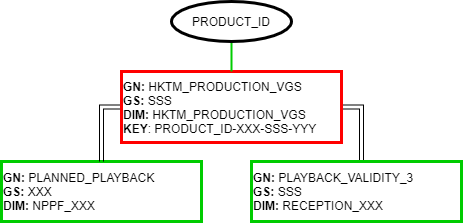
\includegraphics[scale=0.7]{../fig/structure_ingestion_ophktm_events.png}
	\caption{Structure of events inserted by the ingestion module for the OPHKTM file}
	\label{fg:structure_ingestion_ophktm_events}
  \end{center}
\end{figure}

Where XXX is the corresponding satellite id, SSS is the station and YYY is the orbit number.

The table \ref{tb:description_events_ingestion_ophktm} shows the description of the events inserted by the ingestion.

\begin{landscape}
\begin{longtable}{|M{0.15\linewidth}|M{0.05\linewidth}|M{0.10\linewidth}|M{0.10\linewidth}|M{0.15\linewidth}|M{0.15\linewidth}|M{0.15\linewidth}|}
\hline \textbf{Gauge name} & \textbf{Gauge system} & \textbf{DIM signature} & \textbf{Insertion mode} & \textbf{Description} & \textbf{Start} & \textbf{Stop} \\ \hline
\textbf{HKTM\_PRODUCTION\_VGS} & XXX & HKTM\_PRODUCTION\_VGS & EVENT\_KEYS (insert) [KEY: PRODUCT\_ID-XXX-WWW-YYY] & Event for representing the \textbf{generation of the HKTM product} & UTC value inside the generation\_date node & UTC value inside the generation\_date node  \\ \hline
\caption{Table describing the events associated to the ingestion}
\label{tb:description_events_ingestion_ophktm}
\end{longtable}
\end{landscape}

The figure \ref{fg:structure_ingestion_ophktm_annotations} shows a simplified diagram of the structure of annotations inserted (associated structure of values not included for simplicity).

\begin{figure}[H]
  \begin{center}
	\centering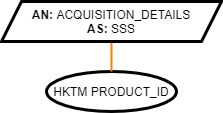
\includegraphics[scale=0.7]{../fig/structure_ingestion_ophktm_annotations.png}
	\caption{Structure of annotations inserted by the ingestion module for the OPHKTM file}
	\label{fg:structure_ingestion_ophktm_annotations}
  \end{center}
\end{figure}

Where SSS is the station.

The table \ref{tb:description_annotations_ingestion_ophktm} shows the description of the annotations inserted by the ingestion.

\begin{longtable}{|M{0.2\linewidth}|M{0.15\linewidth}|M{0.15\linewidth}|M{0.10\linewidth}|M{0.25\linewidth}|}
\hline \textbf{Annotation name} & \textbf{Annotation system} & \textbf{DIM signature} & \textbf{Insertion mode} & \textbf{Description} \\ \hline
\textbf{ACQUISITION\_DETAILS} & SSS & HKTM\_PRODUCTION\_VGS & SIMPLE\_UPDATE (insert) & Annotation for representing the \textbf{acquisition details for the generated HKTM package} \\ \hline
\caption{Table describing the annotations associated to the ingestion}
\label{tb:description_annotations_ingestion_ophktm}
\end{longtable}


